%=========================================================================
% fig-tut3-sort-fl
%=========================================================================

\begin{figure}[b]
  \cbxcaptionsize

  \hfill
  \begin{varwidth}[t]{\tw}
    \vspace{0pt}

    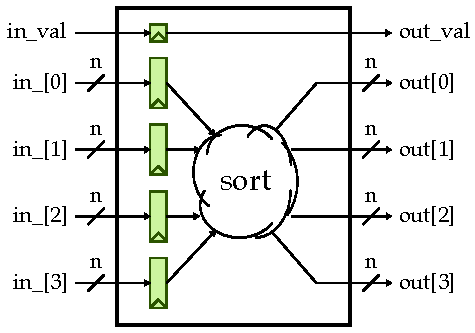
\includegraphics[scale=0.85]{tut3-sort-fl.svg.pdf}

  \end{varwidth}
  \hfill%
  \begin{minipage}[t]{0.44\tw}
    \vspace{0pt}

    \caption{\textbf{Cloud Diagram for Sort Unit FL Model --} Cloud
      diagrams use ``clouds'' to abstractly represent logic without worry
      about the actual implementation details. The sort unit FL model
      takes four input values and sorts them such that the \TT{out[0]}
      port has the smallest value and the \TT{out[1]} port has the
      largest value. Input/output valid bits indicate when the
      input/output values are valid.}
    \label{fig-tut3-sort-fl}

  \end{minipage}
  \hfill\mbox{}

\end{figure}

